\section{Daten}%
\label{sec:daten}
\begin{frame}{Daten}
  \begin{columns}
    \begin{column}[t]{0.5\textwidth}
      \begin{block}{Input}
        \begin{itemize}
          \item Selbstgelabelte Himmelfotos
        \end{itemize}
      \end{block}
    \end{column}
    \begin{column}[t]{0.5\textwidth}
      \begin{block}{Output}
        \begin{itemize}
          \item[\Rightarrow] Wolkentyp
        \end{itemize}
      \end{block}
    \end{column}
  \end{columns}
\end{frame}

\begin{frame}{Input}
  \centering
  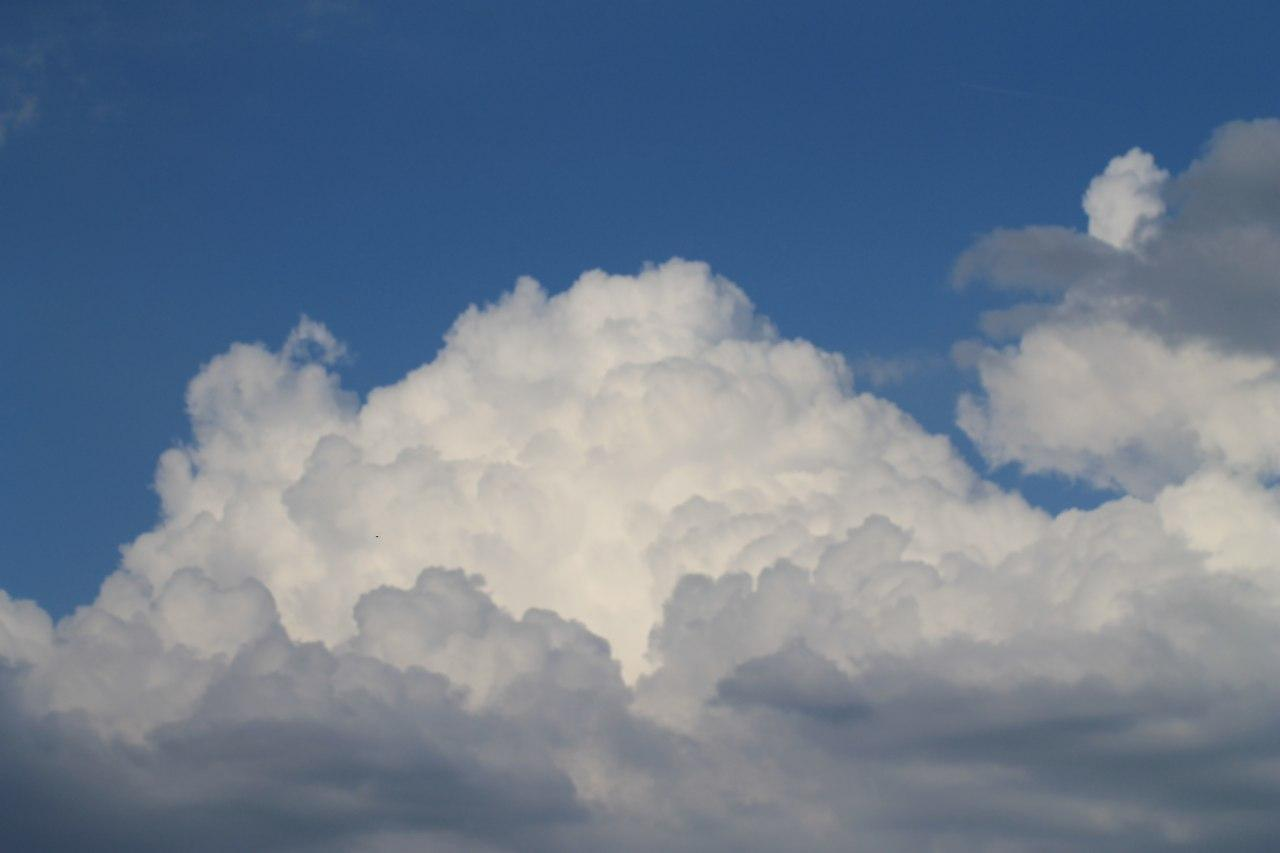
\includegraphics[width=\textwidth]{content/wolke01.jpg}
\end{frame}

\begin{frame}{Output}
  $\Rightarrow$~Cumulonimbus
\end{frame}

\begin{frame}{Wolkentypen}
  \centering
  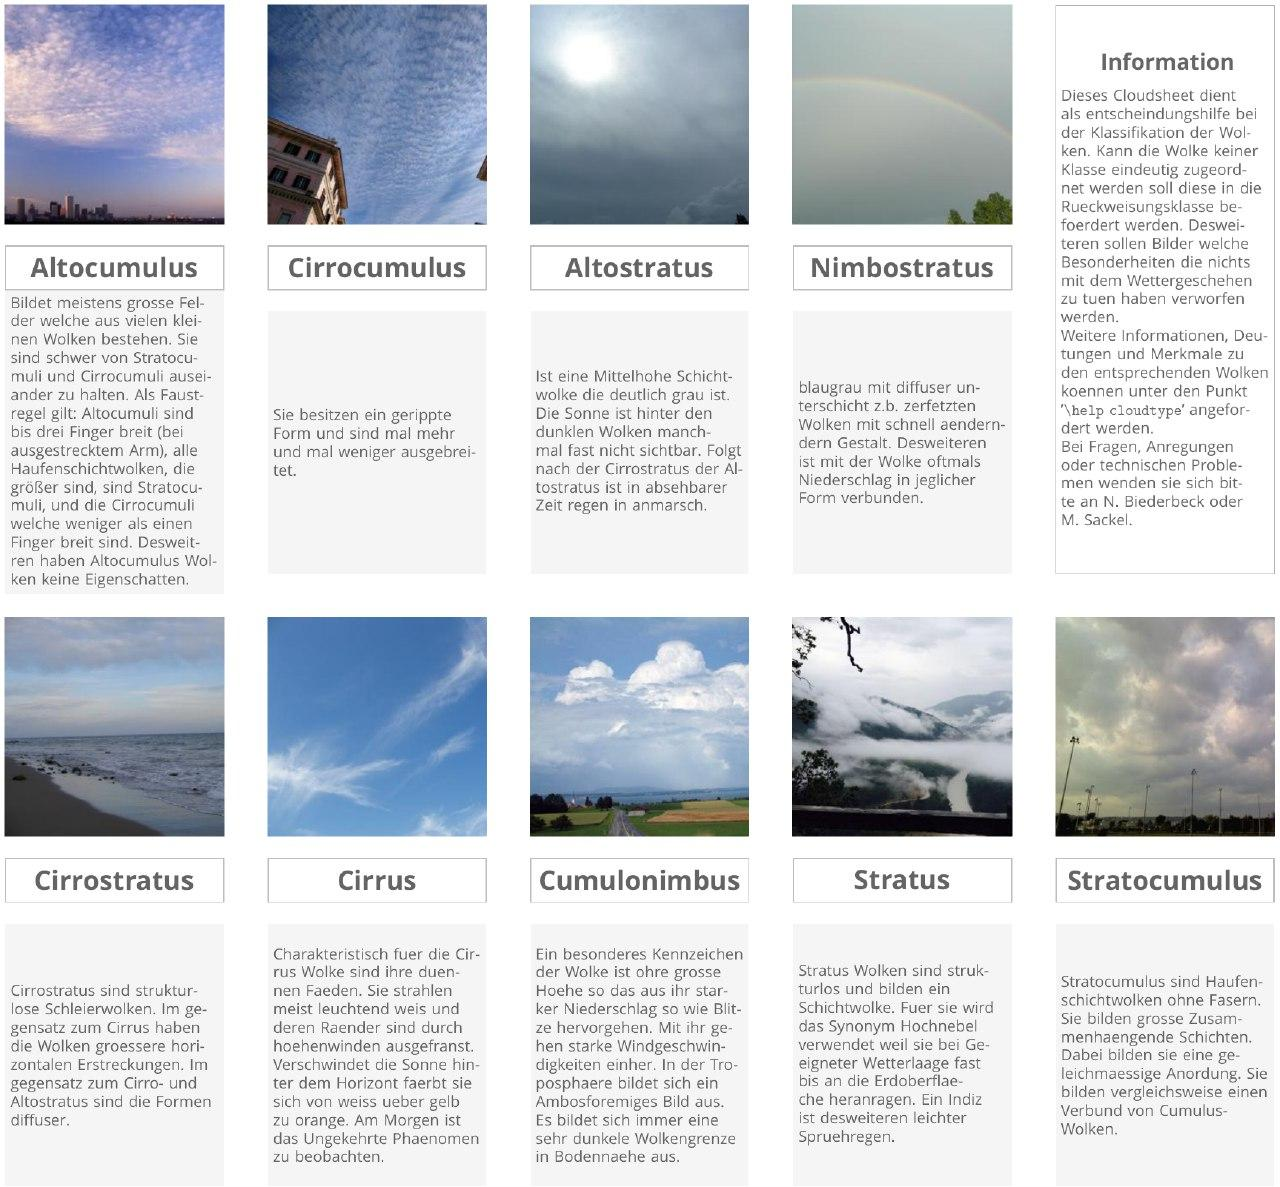
\includegraphics[height=\textheight]{content/cloudsheet.jpg}
\end{frame}
